\chapter{Summary of Chapter 2: The OpenBiodiv Ontology}

\label{chapter-ontology}

OpenBiodiv lifts biodiversity information from scholarly publications and academic databases into a computable semantic form.  In this chapter, we introduce OpenBiodiv-O (\cite{senderov_openbiodiv-o:_2018}), the ontology forming the knowledge and inferencing model of OpenBiodiv. OpenBiodiv-O provides a conceptual model of the structure of a biodiversity publication and the development of related taxonomic concepts. We first introduce the modeled domain in Domain Conceptualization and then formalize it in Results. 

By developing an ontology focusing on biological taxonomy, our intent is to provide an ontology that fills in the gaps between ontologies for biodiversity resources such as Darwin-SW and semantic publishing ontologies such as the ontologies comprising the SPAR Ontologies. We take the view that it is advantageous to model the taxonomic process itself rather than any particular state of knowledge.

The source code and documentation are available under the CC BY license\footnote{Creative Commons Attribution 4.0 International Public License.} from GitHub\footnote{\url{https://github.com/vsenderov/openbiodiv-o/blob/master/LICENSE.md}}. We start by introducing the domain of biological taxonomy and the related biodiversity sciences.

\section{Domain Conceptualization}
We give an introduction of the history of modern biological taxonomy starting with Carl Linnaeus (1707-1778) who proposed the modern organism grouping of \emph{kingdoms, classes, orders, genera} and the usage of Latin binomial names in \emph{Systema Naturae} (\cite{linnaeus_systema_1758}). We emphasize that the work of taxonomists to describe and organize biodiversity is far from complete. This informs the creation of our ontology not as a static formalization of the existing biological taxonomy in computer-readable form, but as a formalization of the \emph{scientific process of biological taxonomy}.

We then describe in the detail what the scientific process of biological taxonomy entails. We start by introducing taxonomic concepts and how they are formed. A taxonomic concept is a scientific hypothesis (\cite{deans_time_2012}) that a certain well-defined group of organisms exists in Nature. It is formed by examining specimens and necessarily entails a scientific grouping criterion, often called a species concept (\cite{mallet_species_2001}; not to be confused with taxonomic concept!). Historically, organisms have been grouped by their appearance (morphological species concept) or reproductive behavior (biological species concept), but recently the focus has shifted towards grouping based on genetic relatedness (phylogenetic and genomic species concepts).

We then describe the ranks of biological taxonomy and how they are regulated by International Codes \cite{international_commission_on_zoological_nomenclature_international_1999,mcneill_international_2012}). The codes govern lower ranks: species, genus, family, order; higher ranks (e.g. phylum, kingdom, domain, etc.) are however free to be used by researchers as they view fit. This leads to multiple competing viewpoints.

Publishing taxonomic concepts is an integral step in the scientific workflow of every taxonomist. We describe the structure and types of taxonomic publications with a particular emphasis on the Treatment section. A Treatment is the section in a taxonomic publication where a taxonomic concept is circumscribed.

\subsection*{Previous work}
We discuss previous efforts made to ontologize  scientific publications and biological information. Particularly important are the Semantic Publishing and Referencing Ontologies (SPAR Ontologies, \cite{peroni_semantic_2014}) and the TaxPub XML Document Type Definition ((\cite{catapano_taxpub:_2010}) referred to loosely as XML schema). The modeling of biodiversity information is primarily influenced by the Codes (\cite{international_commission_on_zoological_nomenclature_international_1999,mcneill_international_2012}), that were mentioned in the previous section, and by a variety of standards (e.g. Darwin Core, DwC, \cite{wieczorek_darwin_2012}), published by the TDWG community.

Finally, we discuss the emerging field of concept taxonomy (\cite{berendsohn_concept_1995, franz_perspectives:_2009,sterner_taxonomy_2017})---a re-imagination of how the circumscription process in biological taxonomy ought to work.

\section{Methods}

OpenBiodiv-O is expressed in Resource Description Framework (RDF). At the onset of the project, a consideration was made to use RDF in favor of a more complex data model such as Neo4J's (\cite{senderov_open_2016}). The choice of RDF was made in order to be able to incorporate the multitude of existing domain ontologies into the overall model.

To develop the conceptualization of the taxonomic process and then the ontology we utilized the following process: (1) domain analysis and identification of important resources and their relationships; (2) analysis of existing data models and ontologies and identification of missing classes and properties for the successful formalization of the domain.

The formal structure of the ontology is specified by employing the RDF Schema (RDFS) and the Web Ontology Language (OWL). It is encoded as a part of a literate programming (\cite{knuth_literate_1984}) document in RMarkdown format titled ``OpenBiodiv Ontology and Guide''\footnote{\href{http://openbiodiv.net/ontology}{http://openbiodiv.net/ontology}}. The statements have been extracted from the RMarkdown file via \emph{knitr} and are provided here as an appendix. It is also possible to request the ontology via Curl from its endpoint with the indication of {\tt content-type: application/rdf+xml}. The vocabularies can be found as additional appendices, Taxonomic Statuses and RCC-5, and on the GitHub page\footnote{\href{https://github.com/vsenderov/openbiodiv-o}{https://github.com/vsenderov/openbiodiv-o}}.

A dataset (OpenBiodiv-LOD, will be described in detail in the next Chapter) from Pensoft's journals, Plazi's treatments, and GBIF's taxonomic backbone has been generated with \mbox{OpenBiodiv-O} and can be found at the SPARQL Endpoint \footnote{\href{http://graph.openbiodiv.net/}{http://graph.openbiodiv.net/}}. The endpoint is also accessible from the website\footnote{\href{http://openbiodiv.net/}{http://openbiodiv.net/}}, under ``SPARQL Endpoint.'' Demos are available as ``Saved Queries'' from the workbench.

\section{Results}

We understand OpenBiodiv-O to be the \emph{shared formal specification of the conceptualization} (\cite{gruber_translation_1993,obitko_translations_2007,staab_handbook_2009}) that we have introduced in Background. OpenBiodiv-O describes the structure of this conceptualization, not any particular state of it.

There are several domains in which the modeled resources fall. The first one is the scholarly biodiversity publishing domain. The second domain is that of taxonomic nomenclature. The third domain is that of broader taxonomic (biodiversity) resources (e.g. taxonomic concepts and their relationships, species occurrences, traits). To combine such disparate resources together we rely on SKOS \cite{miles_skos_nodate}. Unless otherwise noted, the default namespace of the classes and properties for this paper is \url{<http://openbiodiv.net/>}. The prefixes discussed here are listed at the beginning of the ontology source code.

\subsection{Semantic Modeling of the Biodiversity Publishing Domain}

We extend the framework of the SPAR Ontologies by introducing a new class for taxonomic articles, its subsections, as well as a new class for the mentioning of a taxonomic name (see next subsection) in an article. These new classes are summarized in Table~\ref{bibliographic_classes}.

\begin{table}[h!]
\caption{New biodiversity publishing classes introduced.}
      \begin{tabular}{cc}
        \hline
          Class QName             & Comment\\  \hline
  {\tt :Treatment}                & section of a taxonomic article\\
  {\tt :NomenclatureSection}      & subsection of Treatment\\
  {\tt :NomenclatureHeading}      & contains a nomenclatural act \\
  {\tt :NomenclatureCitationList} & list of citations of related concepts\\
  {\tt :MaterialsExamined}        & list of examined specimens\\
  {\tt :BiologySection}           & subsection of Treatment\\
  {\tt :DescriptionSection}       & subsection of Treatment\\
  {\tt :TaxonomicKey}             & section with an identification key\\
  {\tt :TaxonomicChecklist}       & section with a list of taxa for a region\\ 
  {\tt :TaxonomicNameUsage}       & mention of a taxonomic name\\ \hline

      \end{tabular}
      \label{bibliographic_classes}
\end{table}

The classes from this subsection are based on the TaxPub XML Document Type Definition (DTD, also referred to loosely as XML schema, \cite{catapano_taxpub:_2010}), on the structure of Biodiversity Data Journal's
taxonomic paper (\cite{smith_beyond_2013}), and and on the Treatment Ontologies (\cite{catapano_treatment_2016}).

Furthermore, we introduce two properties: \emph{contains} ({\tt :contains}) and \emph{mentions} ({\tt :mentions}). \emph{contains} is used to link parts of the article together and \emph{mentions} links parts of the article to other concepts.

A graphical representation of the relationships between instances of the publishing-related classes that OpenBiodiv introduces is to be found in the diagram in Fig.~\ref{taxonomic-article-diagram}.

\begin{figure}[h!]
	\centering
	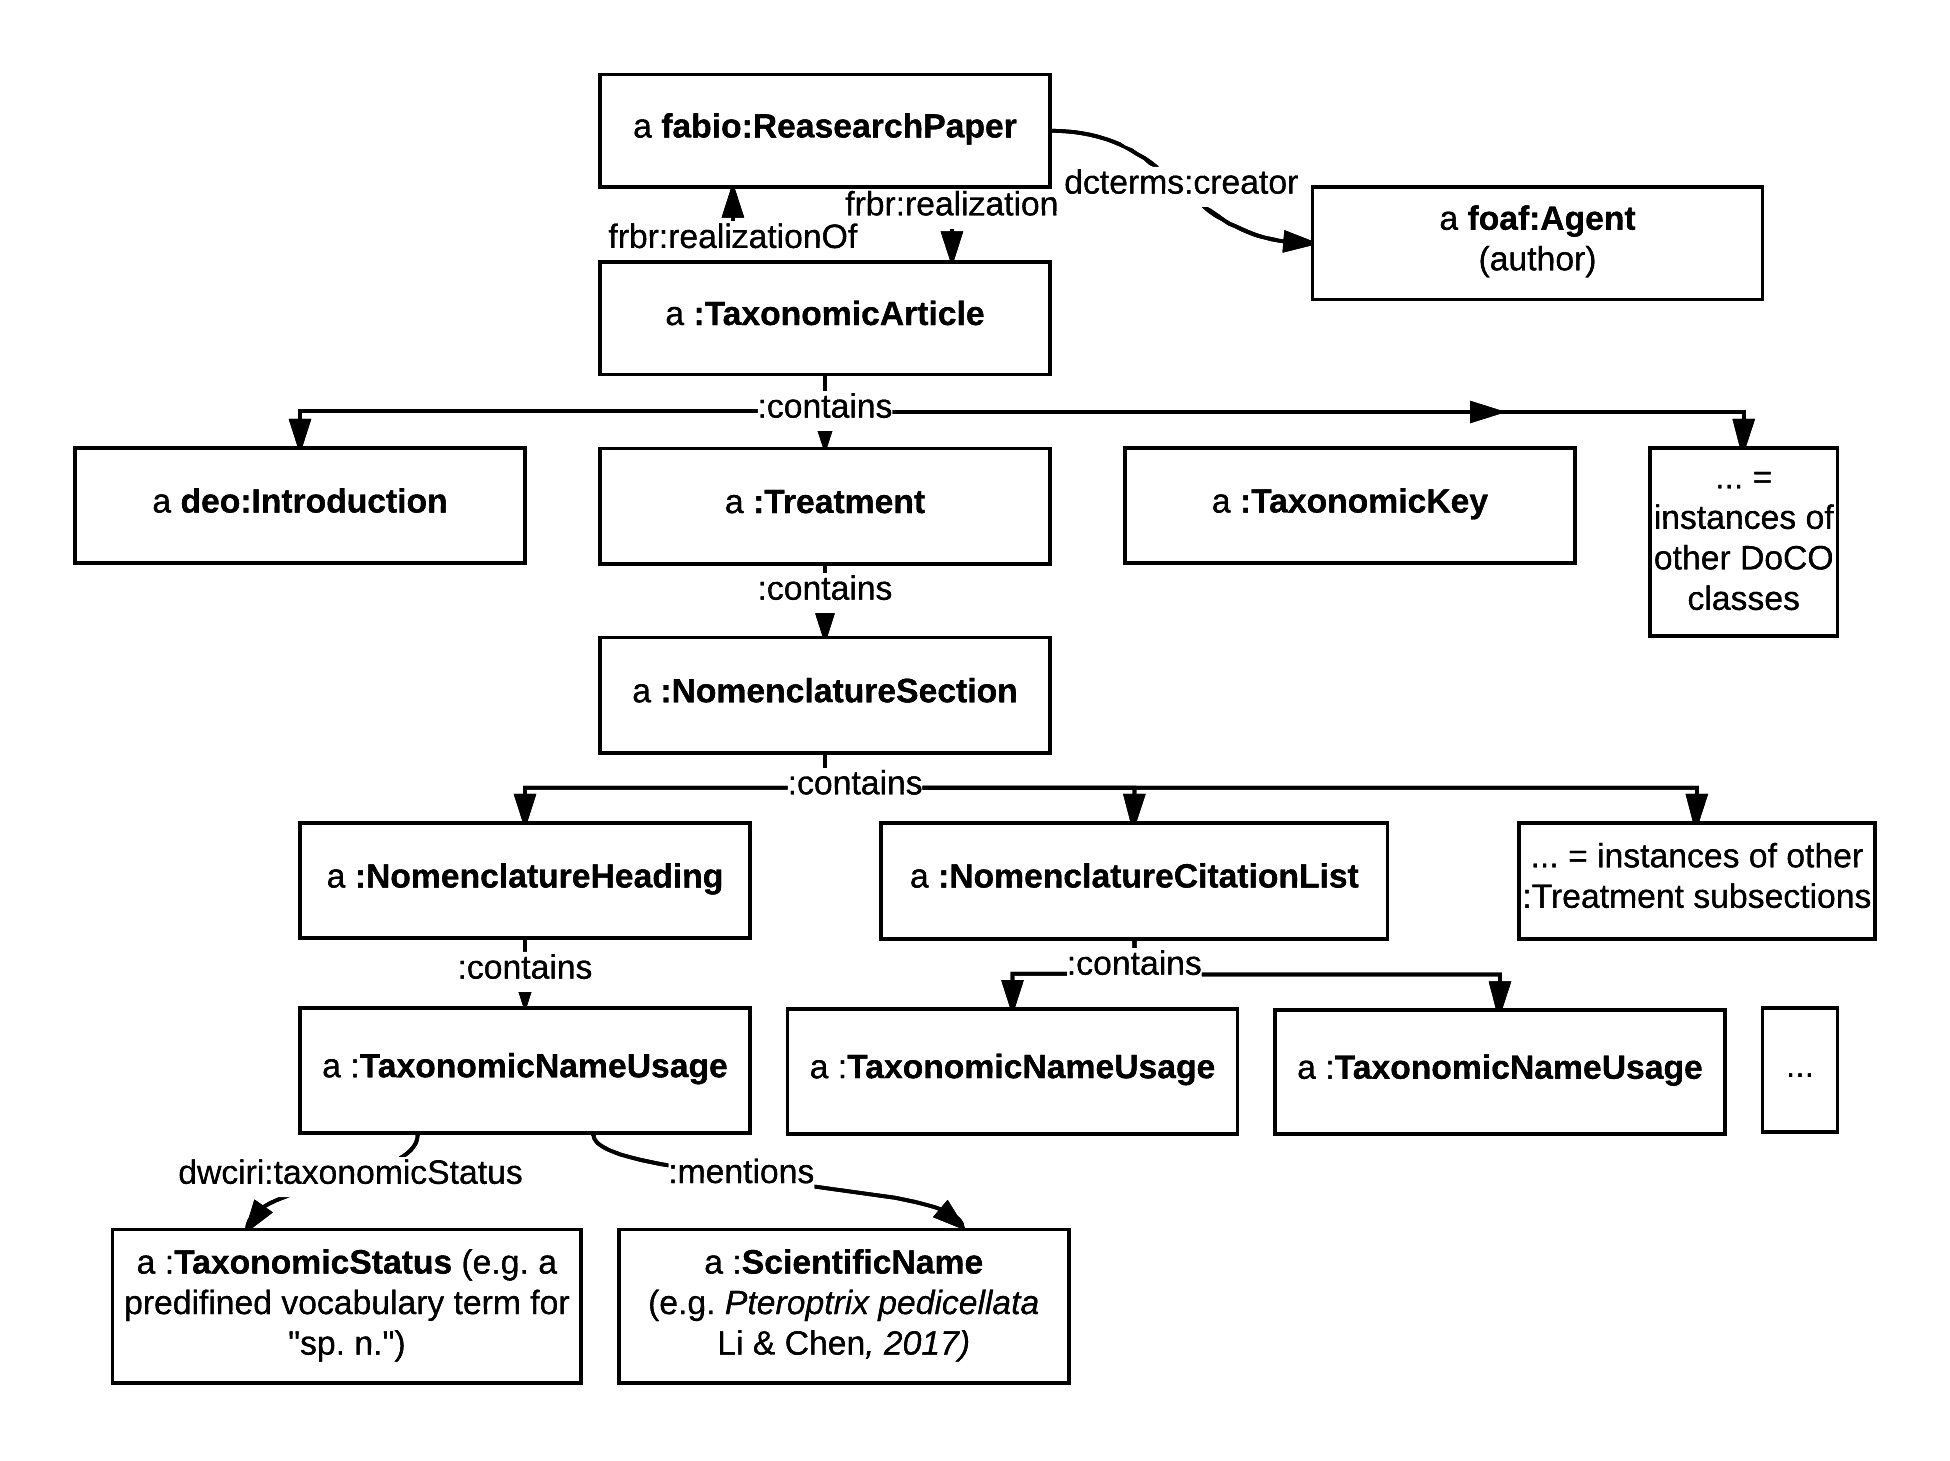
\includegraphics[width=\textwidth]{Figures/taxonomic-article-diagram}
	\decoRule
  \caption[Taxonomic article diagram.]{A graphical representation of the relationships between instances of the publishing-related classes that OpenBiodiv introduces.}
  \label{taxonomic-article-diagram}
\end{figure}

\subsubsection{Semantics, alignment, and usage}

In this section we discuss how the classes and properties that we have introduced align to the Functional Requirements for Bibliographic Records (FRBR) model used by SPAR. In a nutshell taxonomic articles are considered FRBR Expressions of the more abstract FRBR Work that is the intellectual content of the article. Treatments are SPAR discourse elements akin to Introduction, Methods, etc. are also FRBR Expressions. Taxonomic Concepts are their corresponding FRBR Work's.

Figs.~\ref{example-article-metadata} and \ref{example-article-structure} give example usage in Turtle illustrating these ideas.

\begin{figure}[h!]
	\centering
	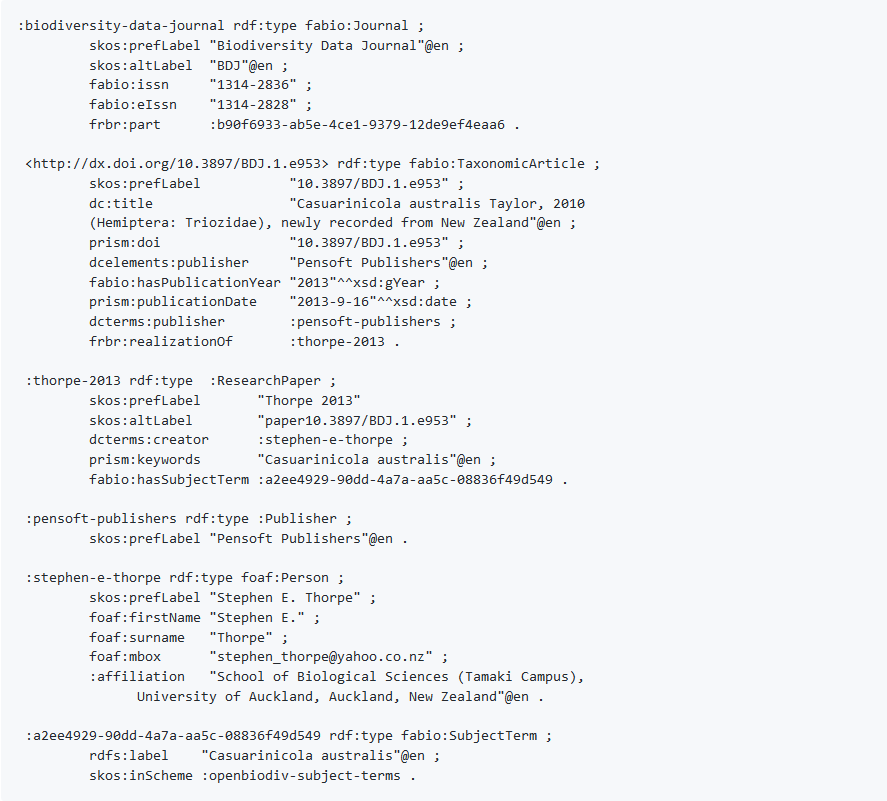
\includegraphics[width=\textwidth]{Figures/example-article-metadata}
	\decoRule
  \caption[Example article metadata.]{This example shows how to express the metadata of a taxonomic article with the SPAR Ontologies' model and the classes that OpenBiodiv defines. The code is in Turtle.}
  \label{example-article-metadata}
\end{figure}

\begin{figure}[h!]
  \centering
  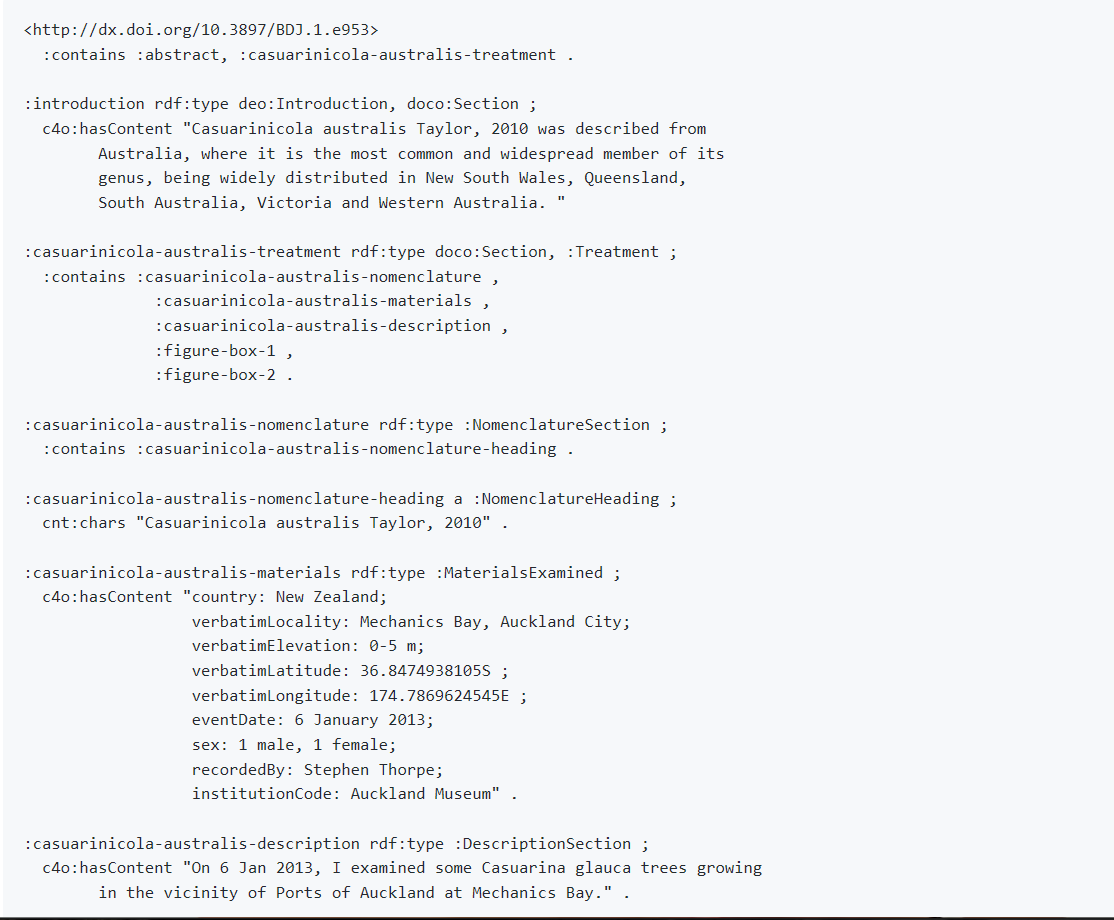
\includegraphics[width=\textwidth]{Figures/example-article-structure}
  \decoRule
  \caption[Example article structure.]{This examples shows how to express the article structure with the help of {\tt :contains}. The code is in Turtle.}
  \label{example-article-structure}
\end{figure}


\subsection{Semantic modeling of biological nomenclature}

Biological nomenclature is a legacy system with over 200 years of accumulation from before the time of informatics and even from before the time of Darwininan Evolution! It is very hard to model due to complexity and has only partially been covered by the ontologies NOMEN and TNSS (introduced in subsection ``Previous work''). With OpenBiodiv-O, I take a bottom-up approach of modeling the use of taxonomic names in articles. Where possible we align OpenBiodiv-O classes to NOMEN.

We have defined the class hierarchy of taxonomic names found in Fig. \ref{taxonomic-name-class-hierarchy-diagram}. Furthermore, we have introduced the class Taxonomic Name Usage ({\tt :TaxonomicNameUsage}). Taxonomic name usages have been discussed widely in the community (e.g. in \cite{pyle_taxonomic_2016}); however, the meaning of term remains vague. The abbreviation TNU is used interchangeably for ``taxon name usage'' and for ``taxonomic name usage.'' In OpenBiodiv-O, a taxonomic name usage is the mentioning of a taxonomic name in the text, optionally followed by a taxonomic status.

\begin{figure}[h!]
  \centering
  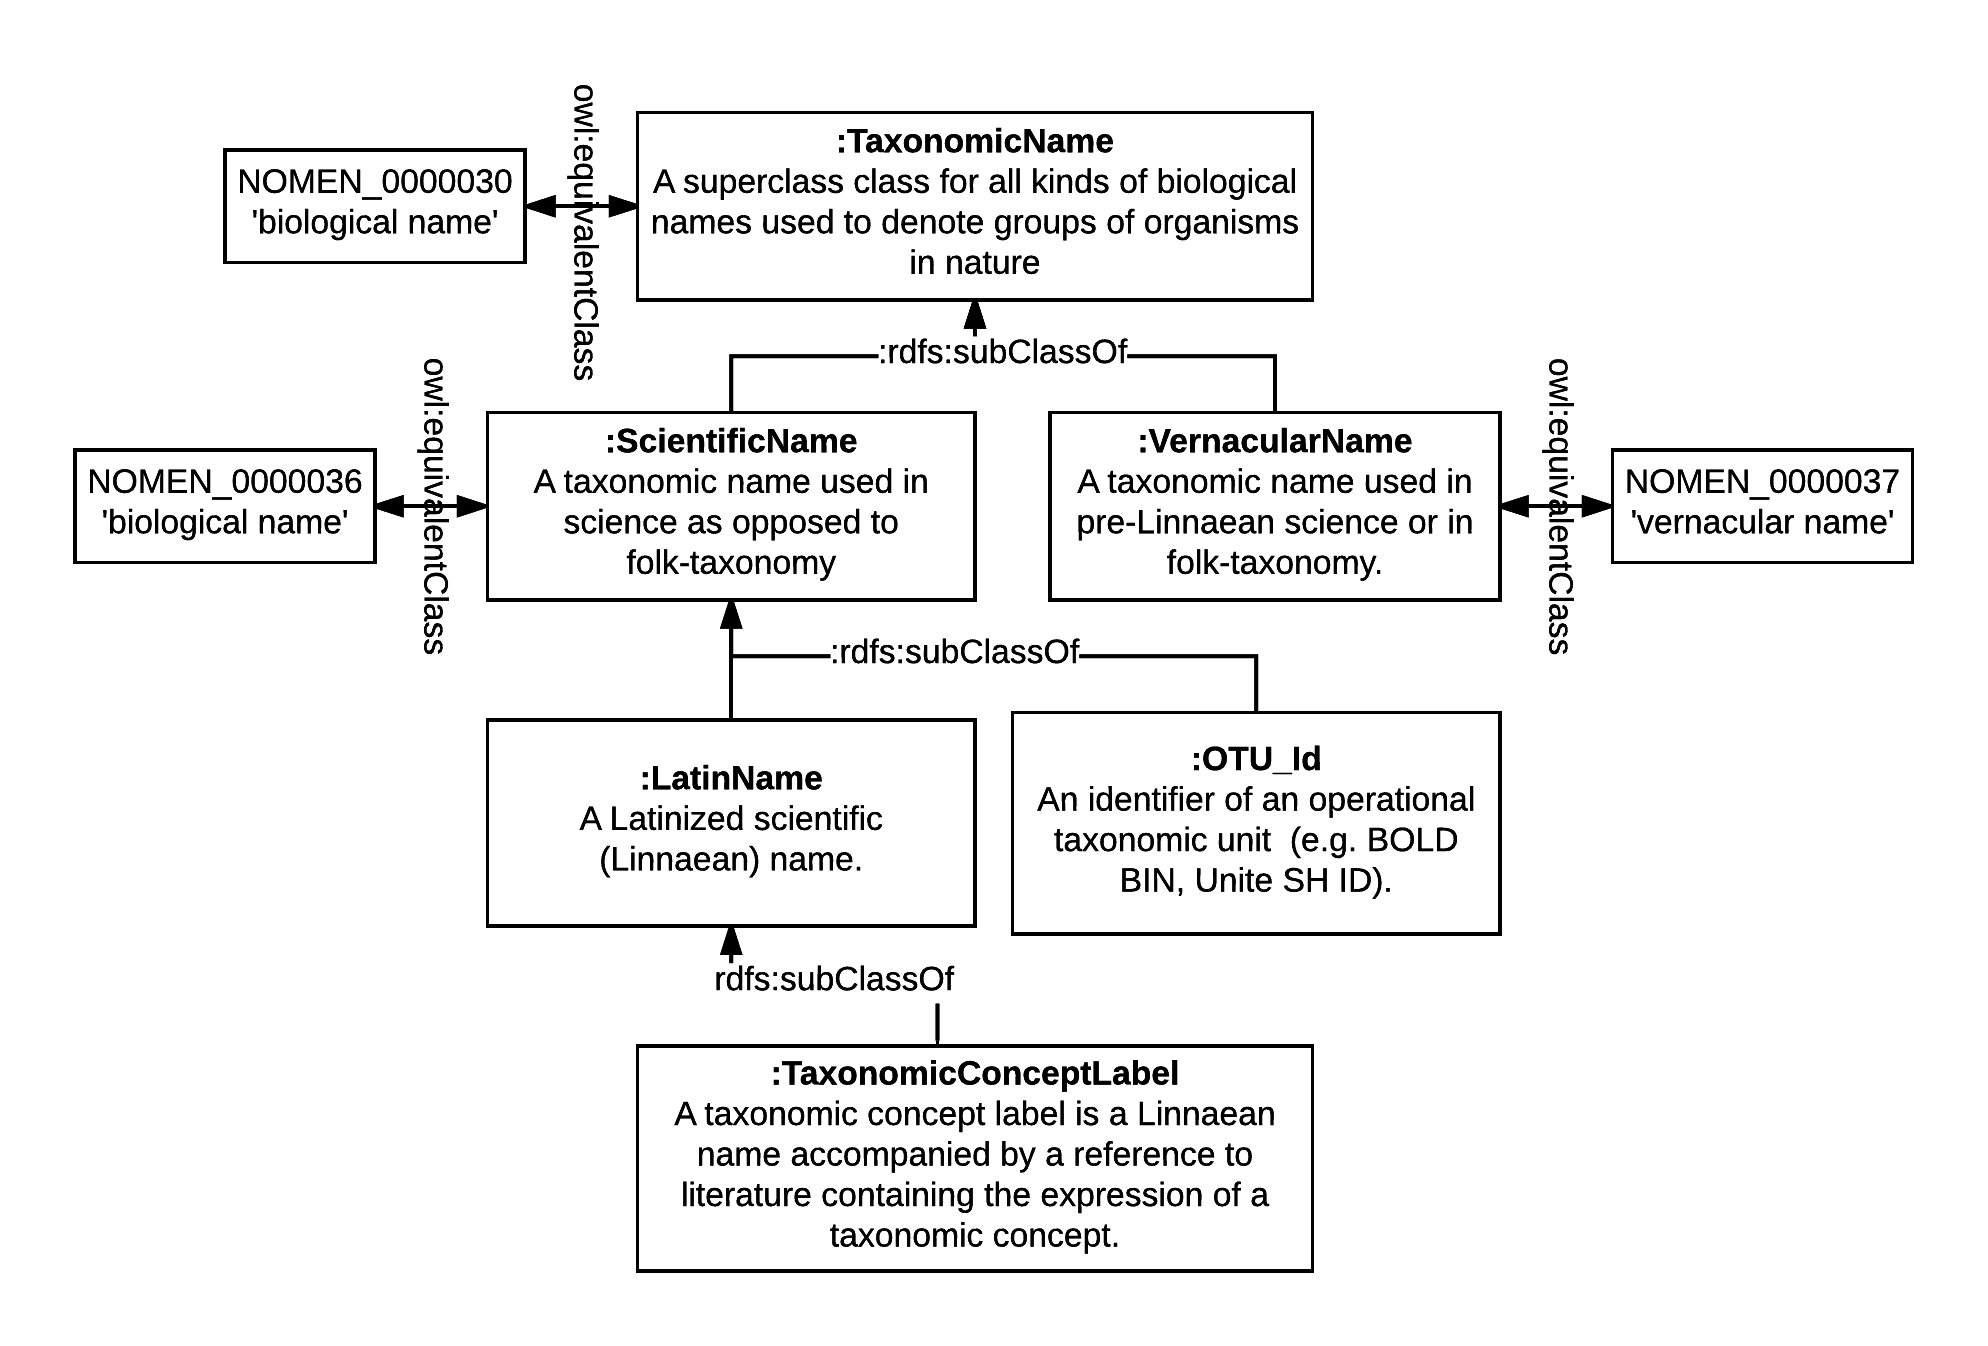
\includegraphics[width=\textwidth]{Figures/taxonomic-name-class-hierarchy-diagram}
  \decoRule
  \caption[Taxonomic name class hierarchy diagram.]{We created this class hierarchy to accommodate both traditional taxonomic name usages and the usage of taxonomic concept labels and operational taxonomic units.}
  \label{taxonomic-name-class-hierarchy-diagram}
\end{figure}

For example, ``\emph{Heser stoevi} Deltschev 2016, sp. n.'' is a taxonomic name usage. The cursive text followed by the author and year of the original species description is the latinized scientific name. The abbreviation ``sp. n.'' stands for the Latin \emph{species novum}, indicating the discovery of a new taxon.

We also introduce the class Taxonomic Concept Label ({\tt :TaxonomicConceptLabel}). A taxonomic concept label (TCL) is a Linnaean name plus a reference to a publication, where the discussed taxon is circumscribed. The link is via the keyword ``sec.'' (Latin for (\emph{secundum}, \cite{berendsohn_concept_1995}). An example would be "\emph{Andropogon virginicus} var. \emph{tenuispatheus} sec. \cite{blomquist_grasses_1948}". Here, \cite{blomquist_grasses_1948} is a valid bibliographic reference to the publication where the concept is circumscribed.

We extracted taxonomic status abbreviations from about 4,000 articles across four taxonomic journals (ZooKeys, Biodiversity Data Journal, PhytoKeys, and MycoKeys) in order to create a taxonomic status vocabulary (see appendices) that covers the eight most common cases (Table \ref{taxonomic-status-vocabulary}). The Latin abbreviations that have been classified into these classes can be found on the OpenBiodiv-O GitHub page. (See Methods for more details).

\begin{table}[h!]
\caption{OpenBiodiv Taxonomic Status Vocabulary.}
\begin{tabular}{ccc}
\hline
Vocabulary Instance QName & Example Abbrev & Comment\\ \hline
{\tt :TaxonomicUncertainty} & \emph{incertae sedis} & Taxonomic Uncertainty\\
{\tt :TaxonDiscovery} & \emph{sp. n.} & Taxonomic Discovery \\
{\tt :ReplacementName} & \emph{comb. n.} & Replacement Name \\
{\tt :UnavailableName} & \emph{nomen dubium} &  Unavailable Name \\
{\tt :AvailableName} & \emph{stat. rev.} & Available Name \\
{\tt :TypeSpecimenDesignation} & \emph{lectotype designation} & Type Specimen Designation \\
{\tt :TypeSpeciesDesignation} & \emph{type species} & Type Species Designation\\
{\tt :NewOccurrenceRecord} & \emph{new country record} & New Occurrence Record (for region)\\
\hline
\end{tabular}
\label{taxonomic-status-vocabulary}
\end{table}

Based on our analysis of taxonomic statuses, we have identified two Code-compliant patterns of relationship between latinized scientific names (Fig. \ref{scientific-name-patterns}). The pattern \emph{replacement name}, implemented via the property {\tt :replacementName}, indicates that a certain Linnaean name should be used instead of another Linnaean name. It covers a wide variety of cases in the Codes, such as, for example, the placement of one species taxon in a new genus ("comb. n."), the correction of a name for nomenclatural reasons ("nomen novum"), or the application of the Principle of Priority for the discovery of synonyms ("syn. nov.", \cite{international_commission_on_zoological_nomenclature_official_2017}).

\begin{figure}[h!]
 \centering
  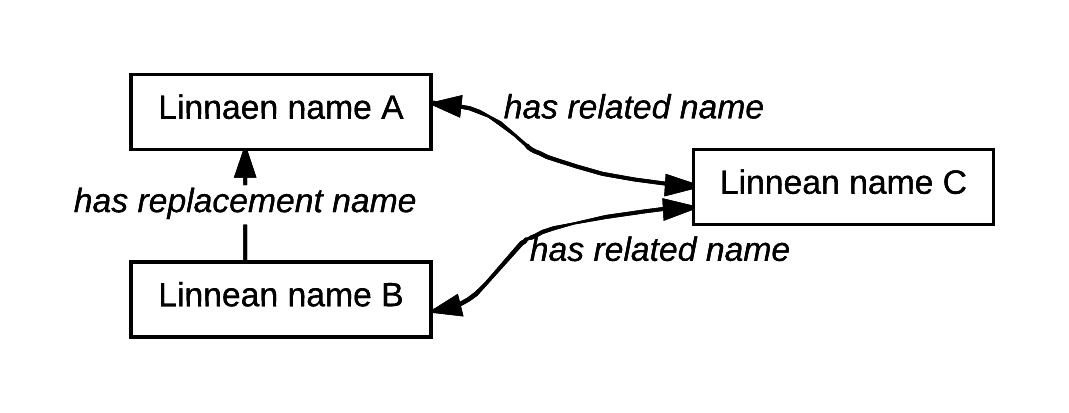
\includegraphics[width=\textwidth]{Figures/scientific-name-patterns}
  \decoRule
  \caption[Scientific name patterns diagram.]{
  Chains of \emph{replacement names} can be followed to find the currently used name. \emph{Related name} indicates that two names are related somehow, but not which one is preferable.}
  \label{scientific-name-patterns}
\end{figure}

The other pattern is that of \emph{related names} ({\tt :relatedName}). It is a broader pattern, indicating that two names are somehow related. For example, they may be synonyms, with one replacing the other, or they may point to taxonomically related taxonomic concepts. For example, \emph{Harmonia manillana} (\cite{mulsant_monographie_1866}) is related to \emph{Caria manillana} \cite{mulsant_monographie_1866} since, as per \cite{poorani_harmonia_2016}, a name-bearing type (lectotype) of \emph{Harmonia manillana} (\cite{mulsant_monographie_1866}) sec. Poorani \cite{poorani_harmonia_2016} is named \emph{Caria manillana} \cite{mulsant_monographie_1866}.

\subsubsection*{Semantics, alignment and usage}
As evident from Fig.~\ref{taxonomic-name-class-hierarchy-diagram}, OpenBiodiv-O taxonomic names are aligned to NOMEN names.

The linking between text and taxonomic names must pass through the intermediary class Taxonomic Name Usage. As parts of the manuscript, taxonomic name usages link document components to taxonomic names. Taxonomic name usages are \emph{contained} in sections such as Treatment, and \emph{mention} a taxonomic name as illustrated in the example in Fig. \ref{example-taxonomic-name-usage}.

\begin{figure}[h!]
\centering
  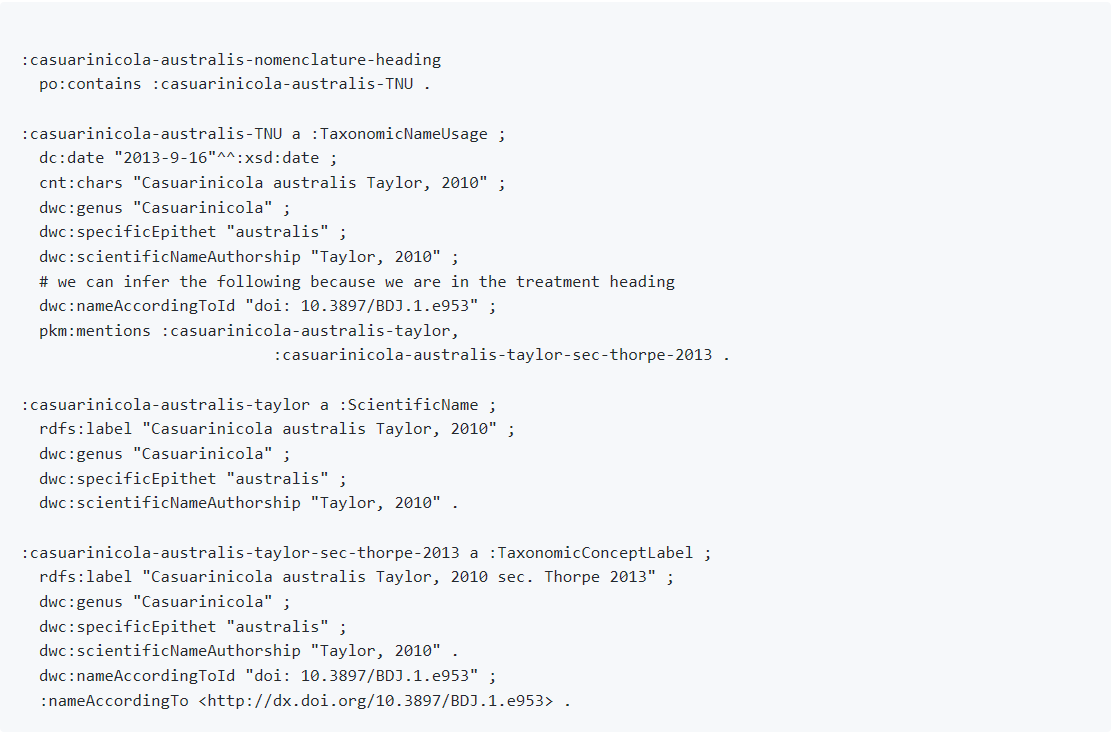
\includegraphics[width=\textwidth]{Figures/example-taxonomic-name-usage}
  \decoRule
  \caption[Example taxonomic name usage.]{
  This examples shows how taxonomic name usages link document components to taxonomic names. The code is in Turtle.}
  \label{example-taxonomic-name-usage}
\end{figure}

\subsection{Semantic Modeling of the Taxonomic Concepts}

In OpenBiodiv-O taxonomic names are not the carriers of semantic information about taxa. This task is accomplished by a new class, Taxonomic Concept ({\tt :TaxonomicConcept}). A taxonomic concept is the theory that a taxonomist forms about a taxon in a scholarly biological taxonomic publication and thus always has a taxonomic concept label. We also introduce a more general class, Operational Taxonomic Unit ({\tt :OperationalTaxonomicUnit}) that can be used for all kinds of taxonomic hypotheses, including ones that don't have a proper taxonomic concept label. The class hierarchy has been illustrated in Fig.~\ref{taxonomic-concept-diagram}.

\begin{figure}[h!]
\centering
  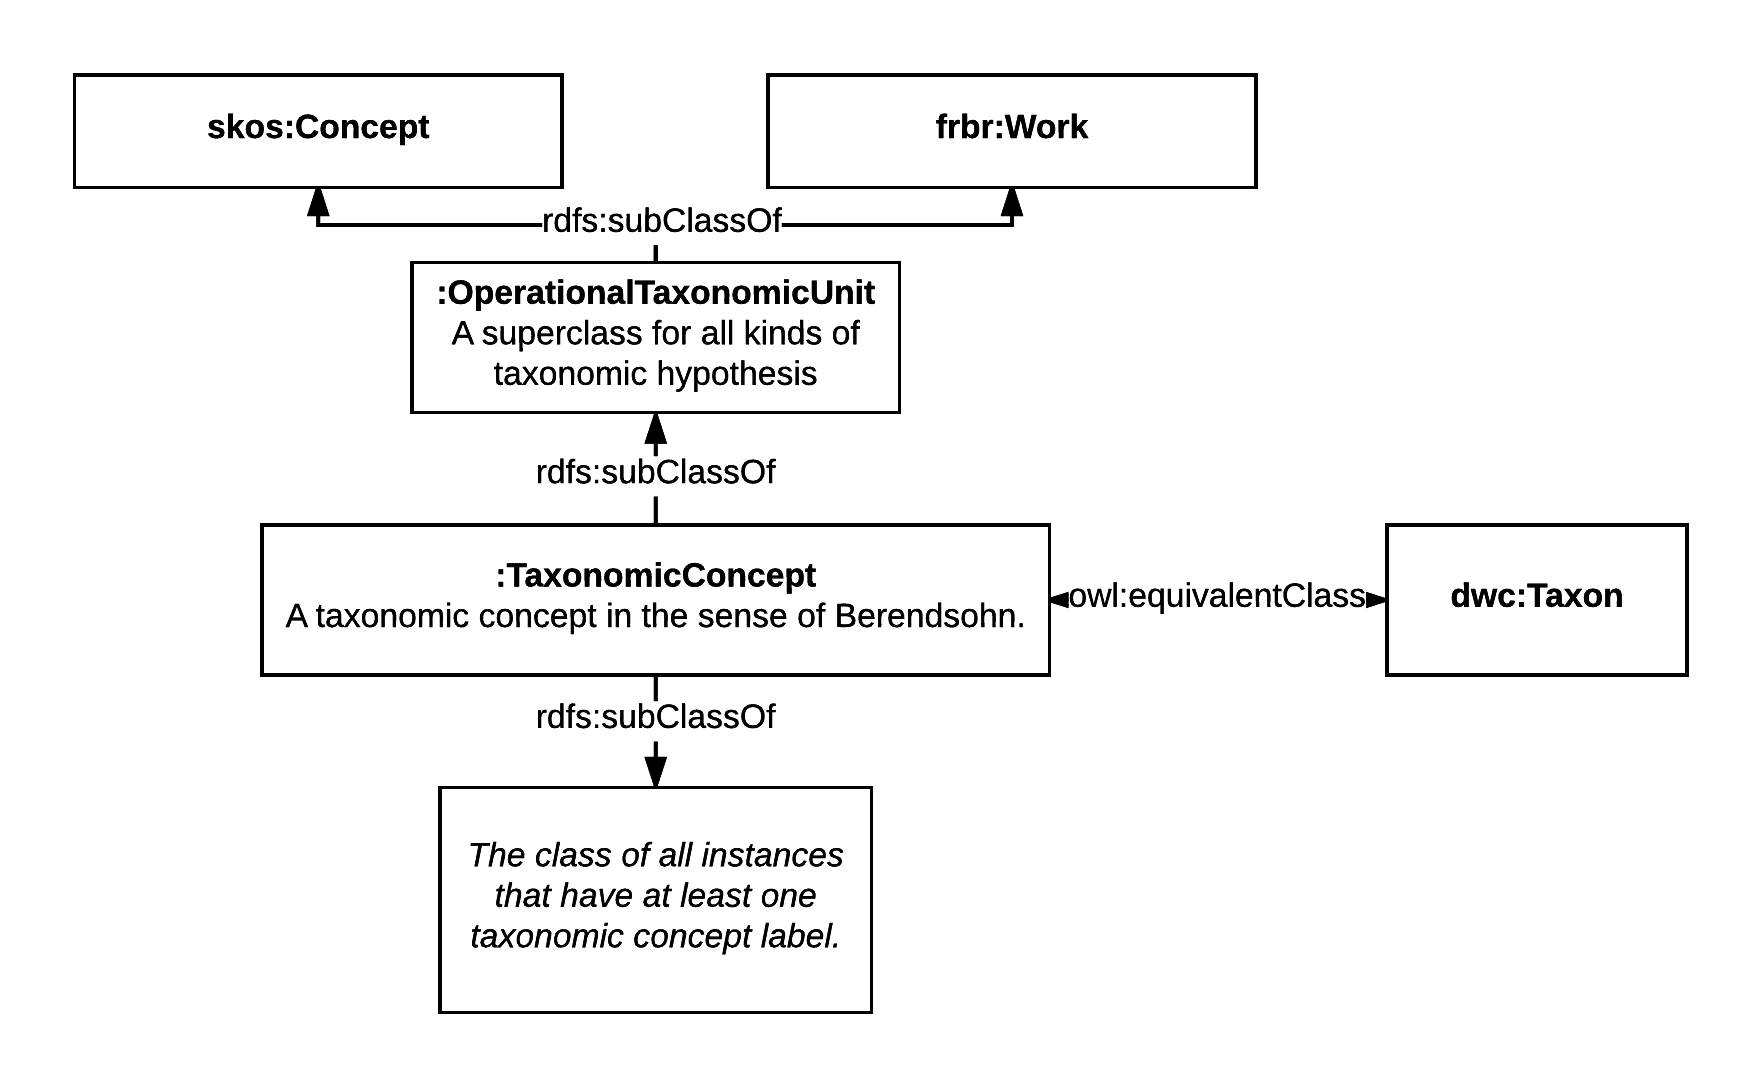
\includegraphics[width=\textwidth]{Figures/taxonomic-concept-diagram}
  \decoRule
  \caption[Taxonomic concept diagram.]{
  A taxonomic concept is a {\tt skos:Concept}, a {\tt frbr:Work}, a {\tt dwc:Taxon} and has at least one taxonomic concept label.}
  \label{taxonomic-concept-diagram}
\end{figure}

Taxonomic concepts are related to taxonomic names---including taxonomic concept labels---via the property \emph{has taxonomic name} ({\tt :taxonomicName}) and its sub-properties mimicking in their range the hierarchy of taxonomic names that we introduced earlier. We have defined a property specifically to link taxonomic concepts to taxonomic concept labels, \emph{has taxonomic concept label} ({\tt :taxonomicConceptLabel}). The property hierarchy diagram is shown in Fig.~\ref{name-property-hierarchy}.

\begin{figure}[h!]
\centering
  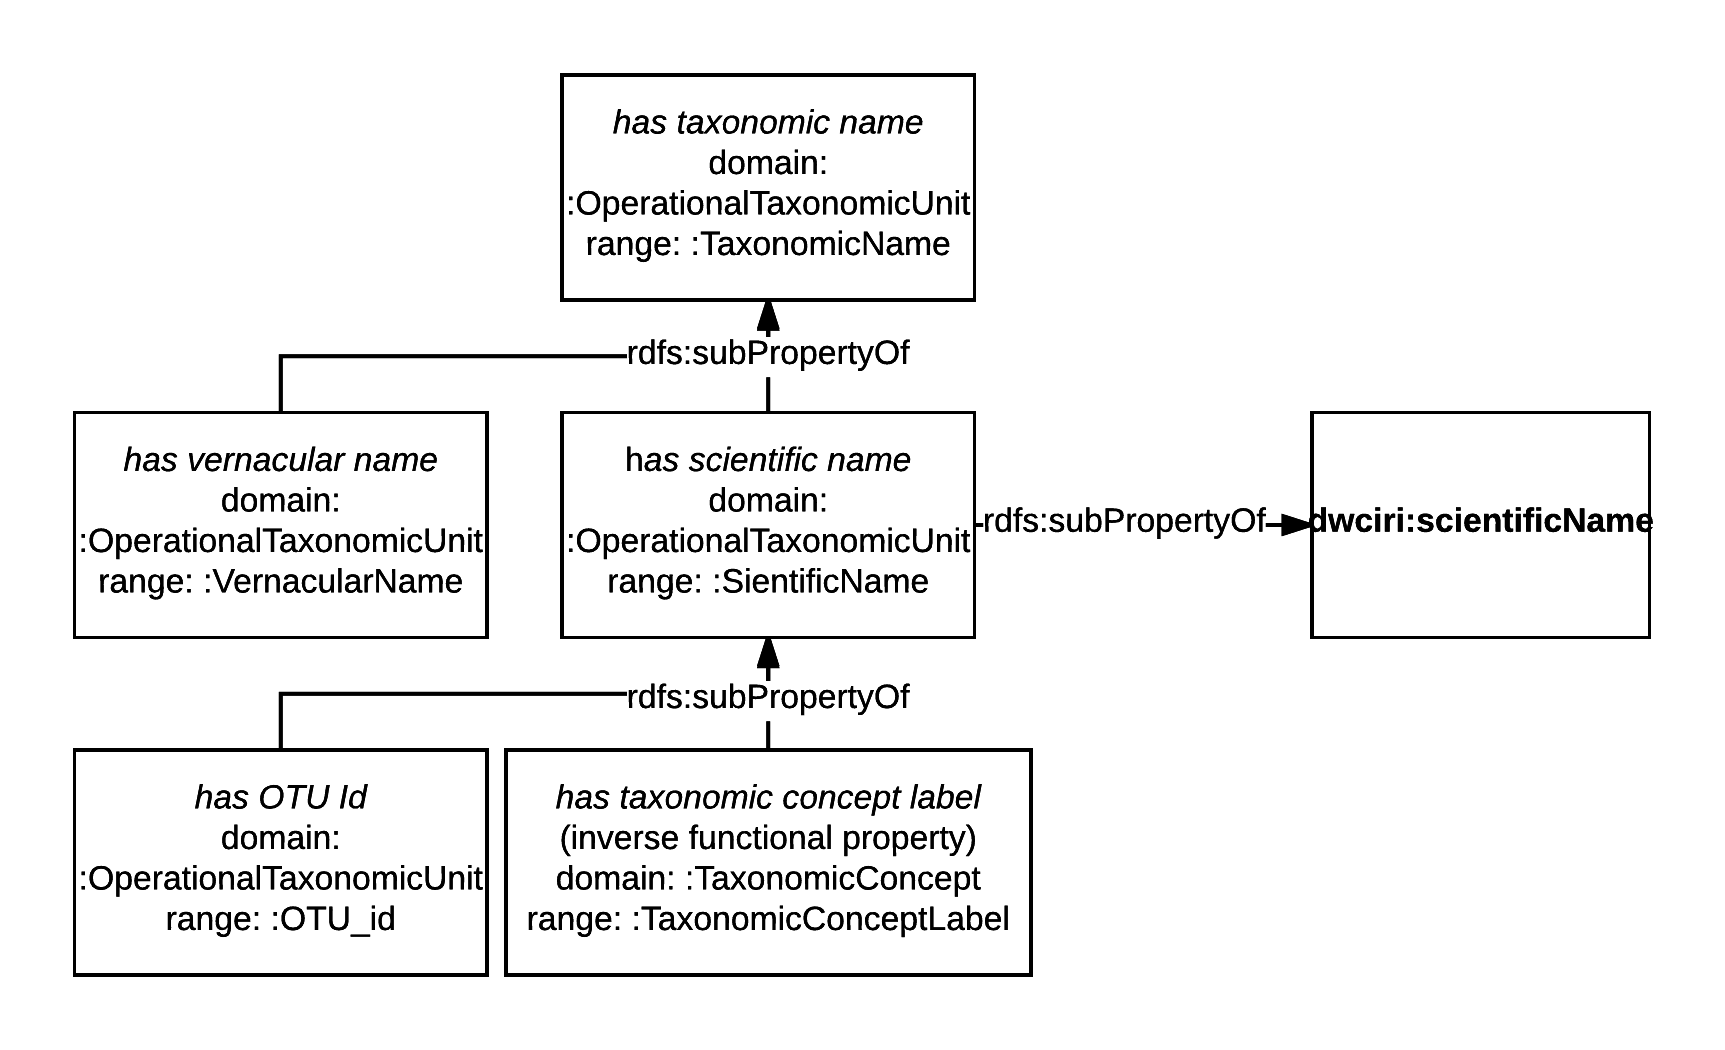
\includegraphics[width=\textwidth]{Figures/name-property-hierarchy}
  \decoRule
  \caption[axonomic name property hierarchy diagram.]
  {Property hierarchy is aligned with the taxonomic name class hierarchy and with DarwinCore.}
  \label{name-property-hierarchy}
\end{figure}

There are two ways to relate taxonomic concepts to each other (Fig. \ref{taxonomic-concept-relationships-diagram}). As we pointed out earlier, historically taxonomic concepts form the hierarchy known as biological taxonomy. To express such simple semantic relations, it is fully sufficient to use the SKOS semantic vocabulary \cite{miles_skos_nodate}. 

\begin{figure}[h!]
\centering
  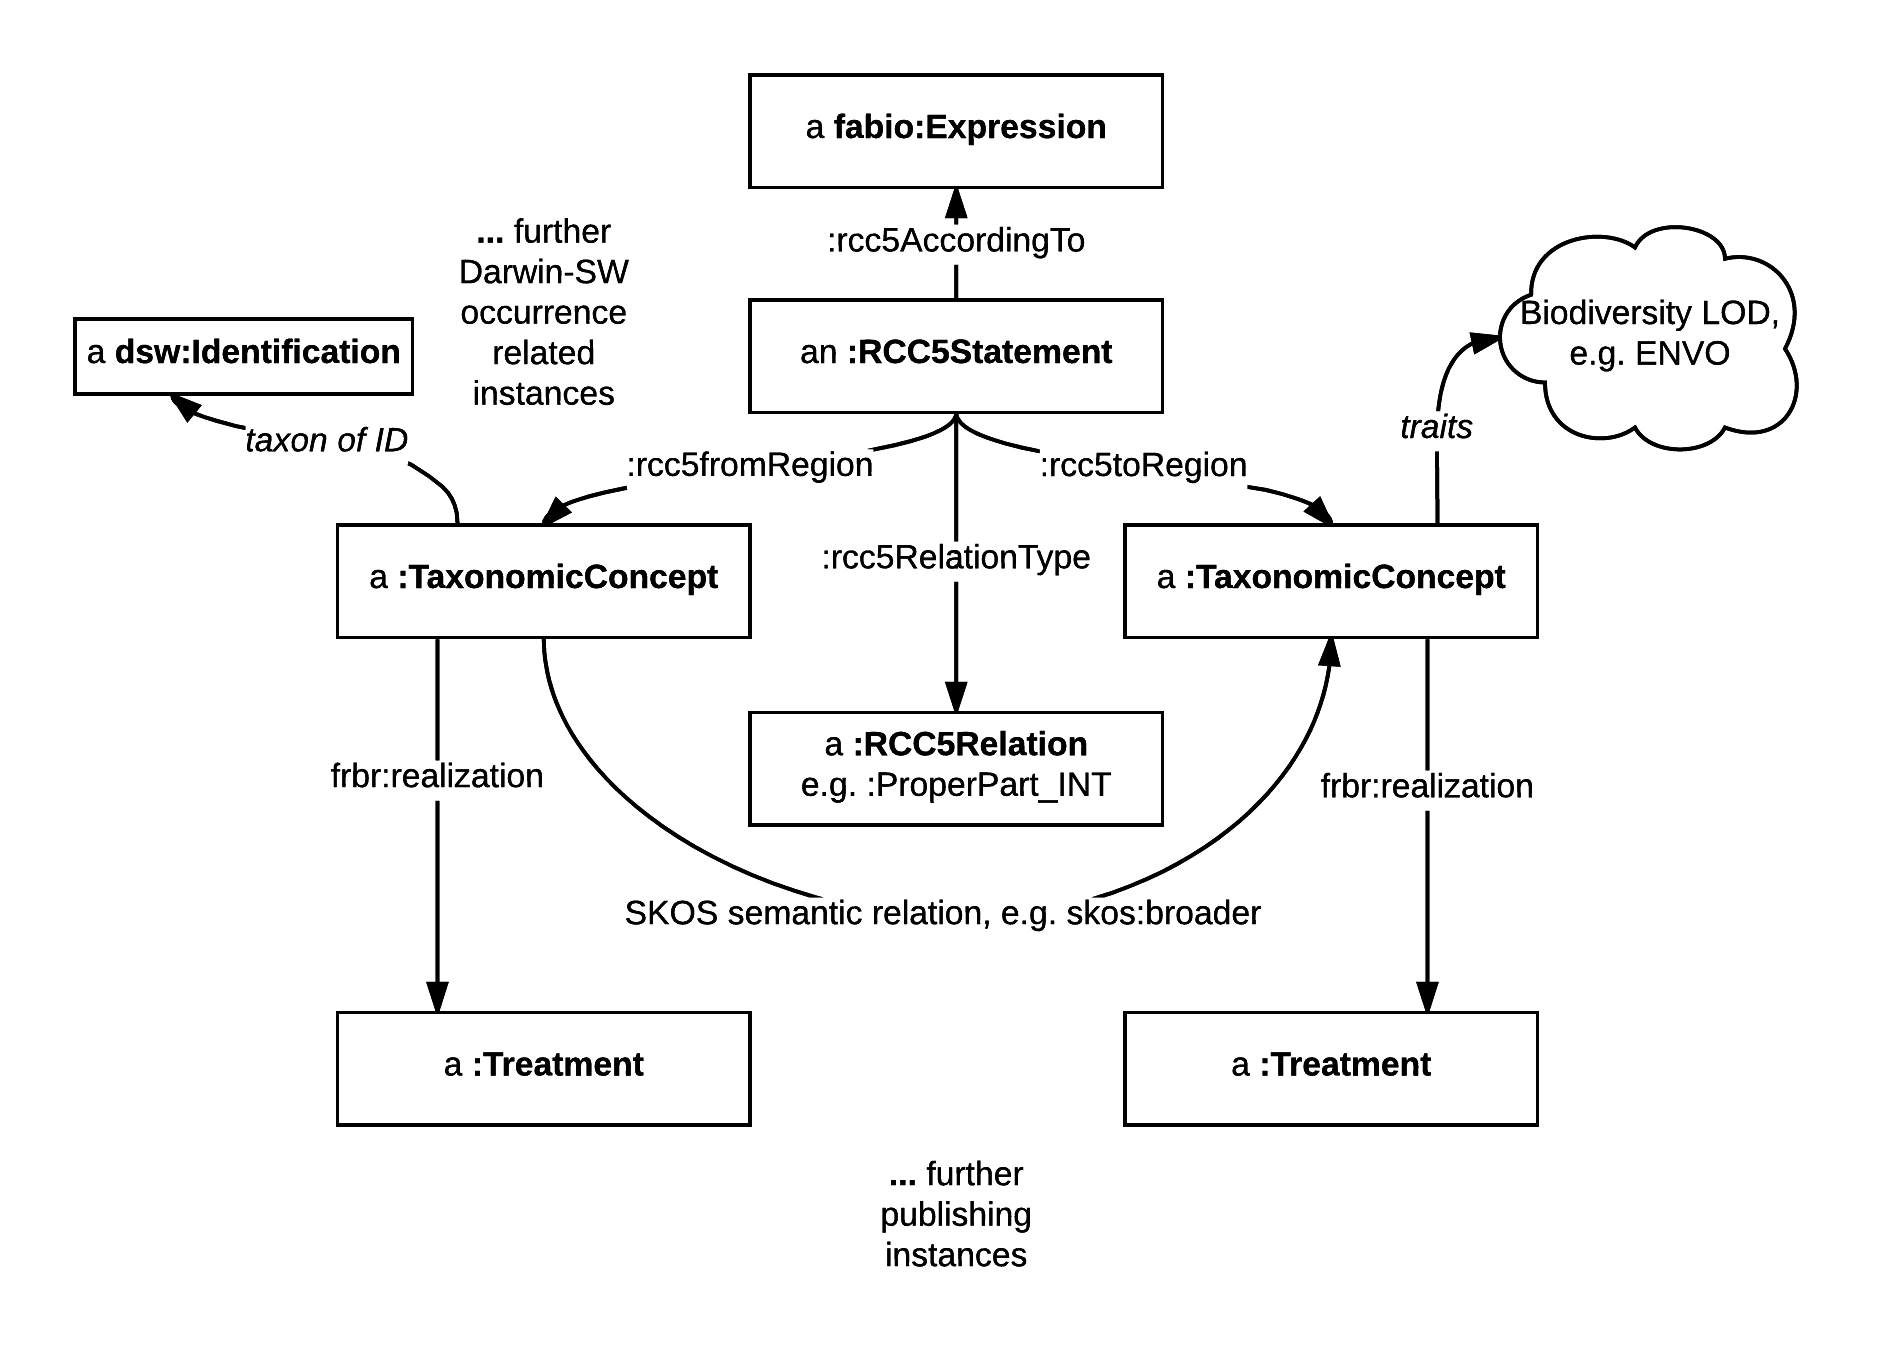
\includegraphics[width=\textwidth]{Figures/taxonomic-concept-relationships-diagram}
  \decoRule
  \caption[Taxonomic concept relationships diagram.]{In order to express an RCC-5 relationship between concepts, create an {\tt :RCC5Sgtatement} and use the corresponding properties to link two taxonomic concepts via it. Further, taxonomic concepts are linked to traits (e.g. ecology in ENVO), occurrences (e.g. Darwin-SW) and realize treatments.}
  \label{taxonomic-concept-relationships-diagram}
\end{figure}

However, these simple relationships are not well suited for machine reasoning. This is why Franz and Peet \cite{franz_perspectives:_2009} suggested, building on previous work by e.g. \cite{koperski_referenzliste_2000}, to use the RCC-5 language to express relationships between taxonomic concepts. Furthermore, the Euler (\cite{chen_euler/x:_2014}) program was developed, which uses Answer Set Programming (ASP) to reason over RCC-5 taxonomic relationships. An answer set reasoner is not part of  OpenBiodiv as this task can be accomplished by Euler; however, we have provided an RCC-5 dictionary class ({\tt :RCC5Dictionary}), an RCC-5 relation term class ({\tt :RCC5Relation}), a vocabulary of such terms to express the RCC-5 relationships in RDF (see appendices), as well as a class and properties to express RCC-5 statements ({\tt :RCC5Statement}, {\tt :rcc5Property}, and subproperties). 

\subsubsection{Semantics and alignment}

In this section taxonomic concepts are aligned to DarwinCore (DwC) and a discussion of how taxonomic concepts related to each either via simple relations (SKOS) and fine-grained (RCC-5) is presented. Also the relationships between biological names and scieintific concepts are discussed. We treat instances of our class Taxonomic Concept as functionally equivalent to DwC Taxa.  We can now list what types of relationships between names and taxonomic concepts are allowed: (1) The relationship between a taxonomic concept and a name that is not a taxonomic concept label is many-to-many---i.e. one Linnaean name can be a mention of multiple taxonomic concepts, and one taxonomic concept may have multiple Linnaean names. (2) The relationship between a taxonomic concept and a taxonomic concept label is one-to-many: while a taxonomic concept may have more than one (at least one is needed) labels, every label uniquely identifies a concept. These logical restrictions make taxonomic concept labels into unique identifiers to taxonomic concepts, something that Linnaean names are not.

\subsubsection{Usage} In Fig. \ref{example-simple-taxonomic-concept-relationships}, Fig.~\ref{example-rcc5-taxonomic-concept-relationships}, and Fig.~\ref{example-envo}, and  Fig~\ref{example-treatment-concept}) we provide some useful examples.

\begin{figure}[h!]
\centering
  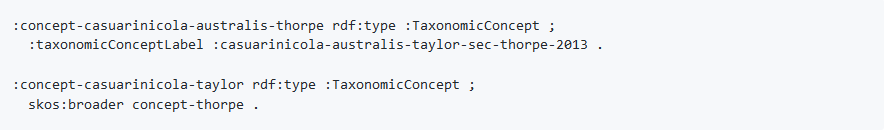
\includegraphics[width=\textwidth]{Figures/example-simple-taxonomic-concept-relationships}
  \decoRule
  \caption[Example simple taxonomic concept relationships.]
  {We can use SKOS semantic properties to illustrate simple relationships between taxonomic concepts.}
  \label{example-simple-taxonomic-concept-relationships}
\end{figure}

\begin{figure}[h!]
\centering
  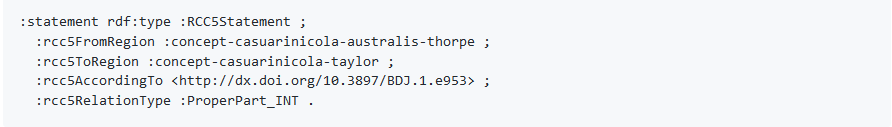
\includegraphics[width=\textwidth]{Figures/example-rcc5-taxonomic-concept-relationships}
  \decoRule
  \caption[Example of RCC-5 taxonomic concept relationships.]{In order to express an RCC-5 relationship between concepts, create an {\tt :RCC5Sgtatement} and use the corresponding properties to link two taxonomic concepts via it. SKOS relations relate concepts directly.}
  \label{example-rcc5-taxonomic-concept-relationships}
\end{figure}


\begin{figure}[h!]
\centering
  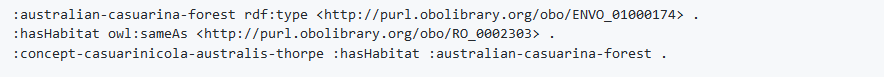
\includegraphics[width=\textwidth]{Figures/example-envo.png}
  \decoRule
  \caption[Example of combining ENVO with OpenBiodiv-O.]{We create a shortcut for \emph{has habitat} and instance of the "forest biome" and link them to our taxonomic concept in order to express the fact that specimens of it have been found to live in \emph{Casuarina} trees.}
  \label{example-envo}
\end{figure}



\begin{figure}[h!]
\centering
  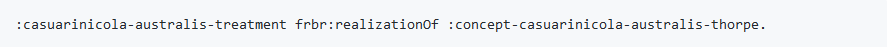
\includegraphics[width=\textwidth]{Figures/example-treatment-concept}
  \decoRule
  \caption[Example connection between a treatment and a taxonomic concept.]{A treatment is the realization of a taxonomic concept.}
  \label{example-treatment-concept}
\end{figure}

\section{Discussion}

OpenBiodiv-O is---together with the Treatment Ontologies (\cite{catapano_treatment_2016})---the first effort to model taxonomic articles as RDF. It introduces classes and properties in the domains of biodiversity publishing and biological taxonomy and aligns them with the SPAR Ontologies, the Treatment Ontologies, the Open Biomedical Ontologies (OBO), TaxPub, NOMEN, and DarwinCore. We believe this introduction bridges the ontological gap that we had outlined in our aims and allows for the creation of a Linked Open Dataset (LOD) of biodiversity information (biodiversity knowledge graph, \cite{senderov_open_2016, page_towards_2016}).

Furthermore, this biodiversity knowledge graph, together with this ontology, additional semantic rules, and user software forms the OpenBiodiv system. OpenBiodiv, as any taxonomic information system should, has taxonomic names as a key building block. For any given taxonomic name, the user will be able to rely on two patterns---\emph{replacement name} and \emph{related name}---to get answers to two questions of high importance to the working taxonomist. First: what is the current and historical usage of any given Linnaean name? Second: given a particular name, what other related names ought to be considered in a taxonomic discussion?

In this section we carry out a discussion how the model of OpenBiodiv can be used to store \emph{multiplicity of opinion} about taxonomic relationships and thus democratize the taxonomic process. We further discuss the usefulness of OpenBiodiv to \emph{answer competency questions} from biological taxonomy. These will be touched upon more in the next chapter.

\section{Conclusions}

The chapter provides an informal conceptualization of the taxonomic process and a formalization in OpenBiodiv-O. It introduces classes and properties in the domains of biodiversity publishing and biological systematics and aligns them with the important domain-specific ontologies. By bridging the ontological gap between the publishing and the biodiversity domains, it will enable the creation of Open Biodiversity Knowledge Management System, consisting of (1) the ontology itself; (2) a Linked Open Dataset (LOD) of biodiversity information (biodiversity knowledge graph); and (3) user interface components aimed at searching, browsing and discovering knowledge in big corpora of previously dispersed scholarly publications. Through the usage of taxonomic concepts, we have included mechanisms for democratization of the scholarly process and not forcing a taxonomic opinion on the users.